> 本章在第五章方向余弦矩阵、第六章相对转动角速度的基础上，给出描述坐标系（刚体）姿态的各类广义坐标：转轴和转角、欧拉参数、欧拉角，以及其他形式（罗德里格斯向量、罗德里格斯参数、修正罗德里格斯参数），并给出这些广义坐标与角速度投影列阵之间的关系及相继转动的合成公式。
\section{转轴和转角}
\subsection{用转轴和转角表示的空间运动刚体角速度}
用转轴和转角表示的方向余弦矩阵为（见第五章）：
\[
\boldsymbol{A}_{ij}=\boldsymbol{I}_3\cos\theta+\tilde{\boldsymbol{n}}\sin\theta+\boldsymbol{n}\boldsymbol{n}^{\mathrm{T}}(1-\cos\theta).
\]
\begin{theorem}[用转轴和转角表示的相对转动角速度]
用转轴和转角表示的相对转动角速度矢量在动系中的投影列阵为

\[
\boldsymbol{\omega}_{ij|j}=\boldsymbol{n}\dot{\theta}+\sin\theta\,\dot{\boldsymbol{n}}-(1-\cos\theta)\tilde{\boldsymbol{n}}\dot{\boldsymbol{n}}.
\]
\end{theorem}
上式两端同时左乘 $\boldsymbol{n}^{\mathrm{T}}$ 可得
\[
\dot{\theta}=\boldsymbol{n}^{\mathrm{T}}\boldsymbol{\omega}_{ij|j}.
\]
回代后可得
\[
\dot{\boldsymbol{n}}=\frac{1}{2\sin\theta}\left[\sin\theta\,\boldsymbol{I}_3-(1+\cos\theta)\tilde{\boldsymbol{n}}\right]\tilde{\boldsymbol{n}}\,\boldsymbol{\omega}_{ij|j}
=\frac{1}{2}\left[\boldsymbol{I}_3-\cot\frac{\theta}{2}\tilde{\boldsymbol{n}}\right]\tilde{\boldsymbol{n}}\,\boldsymbol{\omega}_{ij|j}.
\]
\begin{proof}[推导要点]
左乘 $\boldsymbol{n}^{\mathrm{T}}$ 时利用了单位向量 $\boldsymbol{n}$ 的性质：$\boldsymbol{n}^{\mathrm{T}}\boldsymbol{n}=1$，$\boldsymbol{n}^{\mathrm{T}}\dot{\boldsymbol{n}}=0$（单位向量与其导数正交），$\boldsymbol{n}^{\mathrm{T}}\tilde{\boldsymbol{n}}=\boldsymbol{0}$（$\tilde{\boldsymbol{n}}$ 为 $\boldsymbol{n}$ 的叉乘矩阵，$\boldsymbol{n}\cdot(\boldsymbol{n}\times\cdot)=0$）。将 $\dot{\theta}$ 回代 $\boldsymbol{\omega}_{ij|j}$ 的表达式并化简即得 $\dot{\boldsymbol{n}}$。
\end{proof}
\section{欧拉参数}
方向余弦矩阵与转轴和转角的关系式为
\[
\boldsymbol{A}_{ij}=\boldsymbol{I}_3\cos\theta+\tilde{\boldsymbol{n}}\sin\theta+\boldsymbol{n}\boldsymbol{n}^{\mathrm{T}}(1-\cos\theta).
\]
三角函数的倍角公式：
\[
\cos\theta=2\cos^2\frac{\theta}{2}-1,\qquad
\sin\theta=2\cos\frac{\theta}{2}\sin\frac{\theta}{2},\qquad
(1-\cos\theta)=2\sin^2\frac{\theta}{2}.
\]
\begin{definition}[欧拉参数]
定义四个欧拉参数为

\[
\left[\varepsilon_1\quad\varepsilon_2\quad\varepsilon_3\right]^{\mathrm{T}}\triangleq\boldsymbol{n}\sin\frac{\theta}{2}=:\bar{\boldsymbol{\varepsilon}},\qquad
\varepsilon_4\triangleq\cos\frac{\theta}{2}.
\]

四个欧拉参数满足模为 1 的约束方程：

\[
\bar{\boldsymbol{\varepsilon}}^2+\varepsilon_4^2=\boldsymbol{n}^2\sin^2\frac{\theta}{2}+\cos^2\frac{\theta}{2}=\sin^2\frac{\theta}{2}+\cos^2\frac{\theta}{2}=1,
\]

即

\[
\varepsilon_1^2+\varepsilon_2^2+\varepsilon_3^2+\varepsilon_4^2=1.
\]
\end{definition}
用欧拉参数表示的方向余弦矩阵形式不唯一：
\begin{theorem}[欧拉参数表示的方向余弦矩阵]
\[
\begin{cases}
\boldsymbol{A}_{ij}=\boldsymbol{I}_3(2\varepsilon_4^2-1)+2\tilde{\bar{\boldsymbol{\varepsilon}}}\varepsilon_4+2\bar{\boldsymbol{\varepsilon}}\bar{\boldsymbol{\varepsilon}}^{\mathrm{T}},\\
\boldsymbol{A}_{ij}=\boldsymbol{I}_3(1-2\bar{\boldsymbol{\varepsilon}}^2)+2\tilde{\bar{\boldsymbol{\varepsilon}}}\varepsilon_4+2\bar{\boldsymbol{\varepsilon}}\bar{\boldsymbol{\varepsilon}}^{\mathrm{T}},
\end{cases}
\]

其中 $\tilde{\bar{\boldsymbol{\varepsilon}}}$ 为 $\bar{\boldsymbol{\varepsilon}}$ 的叉乘矩阵。展开得

\[
\boldsymbol{A}_{ij}=
\begin{bmatrix}
1-2\varepsilon_2^2-2\varepsilon_3^2 & 2(\varepsilon_1\varepsilon_2-\varepsilon_3\varepsilon_4) & 2(\varepsilon_1\varepsilon_3+\varepsilon_2\varepsilon_4)\\
2(\varepsilon_2\varepsilon_1+\varepsilon_3\varepsilon_4) & 1-2\varepsilon_3^2-2\varepsilon_1^2 & 2(\varepsilon_2\varepsilon_3-\varepsilon_1\varepsilon_4)\\
2(\varepsilon_3\varepsilon_1-\varepsilon_2\varepsilon_4) & 2(\varepsilon_3\varepsilon_2+\varepsilon_1\varepsilon_4) & 1-2\varepsilon_1^2-2\varepsilon_2^2
\end{bmatrix}.
\]
\end{theorem}
由 $\tilde{\boldsymbol{\omega}}_{ij|j}=\boldsymbol{A}_{ij}^{\mathrm{T}}\dot{\boldsymbol{A}}_{ij}$，可得用欧拉参数及其导数表示的 $\boldsymbol{\omega}_{ij|j}$ 的表达式。
\begin{theorem}[欧拉参数表示的角速度]
\[
\boldsymbol{\omega}_{ij|j}=2
\begin{bmatrix}
\varepsilon_4 & \varepsilon_3 & -\varepsilon_2 & -\varepsilon_1\\
-\varepsilon_3 & \varepsilon_4 & \varepsilon_1 & -\varepsilon_2\\
\varepsilon_2 & -\varepsilon_1 & \varepsilon_4 & -\varepsilon_3
\end{bmatrix}
\begin{bmatrix}
\dot{\varepsilon}_1\\ \dot{\varepsilon}_2\\ \dot{\varepsilon}_3\\ \dot{\varepsilon}_4
\end{bmatrix}
=2\left[\varepsilon_4\boldsymbol{I}_3-\tilde{\bar{\boldsymbol{\varepsilon}}}\quad -\bar{\boldsymbol{\varepsilon}}\right]\dot{\boldsymbol{\varepsilon}}
=:\boldsymbol{H}_{\mathrm{EP}}\dot{\boldsymbol{\varepsilon}}.
\]
\end{theorem}
进一步可得 $\boldsymbol{\omega}_{ij|j}$ 在 $i$ 系中的投影列阵：
\[
\boldsymbol{\omega}_{ij|i}=\boldsymbol{A}_{ij}\boldsymbol{\omega}_{ij|j}
=2\left[\varepsilon_4\boldsymbol{I}_3+\tilde{\bar{\boldsymbol{\varepsilon}}}\quad -\bar{\boldsymbol{\varepsilon}}\right]\dot{\boldsymbol{\varepsilon}}.
\]
\begin{proof}[推导过程]
以 $x$ 分量为例：

\[
\begin{aligned}
(\omega_x)_{ij|j} &= a_{13}\dot{a}_{12}+a_{23}\dot{a}_{22}+a_{33}\dot{a}_{32}\\
&= \left[4\varepsilon_1(\varepsilon_1\varepsilon_4-\varepsilon_2\varepsilon_3)+2\varepsilon_4\right]\dot{\varepsilon}_1
+ \left[4\varepsilon_2(\varepsilon_1\varepsilon_4-\varepsilon_2\varepsilon_3)+2\varepsilon_3\right]\dot{\varepsilon}_2\\
&\quad + \left[4\varepsilon_3(\varepsilon_1\varepsilon_4-\varepsilon_2\varepsilon_3)-2\varepsilon_2\right]\dot{\varepsilon}_3
+ \left[4\varepsilon_4(\varepsilon_1\varepsilon_4-\varepsilon_2\varepsilon_3)-2\varepsilon_1\right]\dot{\varepsilon}_4\\
&= 2\varepsilon_4\dot{\varepsilon}_1+2\varepsilon_3\dot{\varepsilon}_2-2\varepsilon_2\dot{\varepsilon}_3-2\varepsilon_1\dot{\varepsilon}_4.
\end{aligned}
\]

化简时利用了约束方程 $1=\varepsilon_1^2+\varepsilon_2^2+\varepsilon_3^2+\varepsilon_4^2$ 及其导数

\[
0=2(\varepsilon_1\dot{\varepsilon}_1+\varepsilon_2\dot{\varepsilon}_2+\varepsilon_3\dot{\varepsilon}_3+\varepsilon_4\dot{\varepsilon}_4),
\]

即中间含因子 $4(\varepsilon_1\varepsilon_4-\varepsilon_2\varepsilon_3)(\varepsilon_1\dot{\varepsilon}_1+\varepsilon_2\dot{\varepsilon}_2+\varepsilon_3\dot{\varepsilon}_3+\varepsilon_4\dot{\varepsilon}_4)$ 的各项之和为零。$y$、$z$ 分量同理。
\end{proof}
\begin{proof}[说明]
若将 $\boldsymbol{\omega}_{ij|j}$ 显式写成 $\boldsymbol{\varepsilon}$ 的线性形式（把 $\dot{\boldsymbol{\varepsilon}}$ 视为独立变量），其系数矩阵为

\[
\frac{\partial\boldsymbol{\omega}_{ij|j}}{\partial\boldsymbol{\varepsilon}}
=2
\begin{bmatrix}
-\dot{\varepsilon}_4 & -\dot{\varepsilon}_3 & \dot{\varepsilon}_2 & \dot{\varepsilon}_1\\
\dot{\varepsilon}_3 & -\dot{\varepsilon}_4 & -\dot{\varepsilon}_1 & \dot{\varepsilon}_2\\
-\dot{\varepsilon}_2 & \dot{\varepsilon}_1 & -\dot{\varepsilon}_4 & \dot{\varepsilon}_3
\end{bmatrix}
=2\left[-\dot{\varepsilon}_4\boldsymbol{I}_3+\tilde{\dot{\bar{\boldsymbol{\varepsilon}}}}\quad \dot{\bar{\boldsymbol{\varepsilon}}}\right].
\]

（注：教材原书将此矩阵标注为 $\partial\boldsymbol{\omega}_{ij|i}/\partial\boldsymbol{\varepsilon}$，经核对应为 $\partial\boldsymbol{\omega}_{ij|j}/\partial\boldsymbol{\varepsilon}$，即 $j$ 系中的投影列阵。）
\end{proof}
\subsection{由角速度列阵反求欧拉参数对时间的一阶导数}
用欧拉参数及其导数表示的 $\boldsymbol{\omega}_{ij|j}$ 的表达式为
\[
\boldsymbol{\omega}_{ij|j}=2
\begin{bmatrix}
\varepsilon_4 & \varepsilon_3 & -\varepsilon_2 & -\varepsilon_1\\
-\varepsilon_3 & \varepsilon_4 & \varepsilon_1 & -\varepsilon_2\\
\varepsilon_2 & -\varepsilon_1 & \varepsilon_4 & -\varepsilon_3
\end{bmatrix}
\begin{bmatrix}
\dot{\varepsilon}_1\\ \dot{\varepsilon}_2\\ \dot{\varepsilon}_3\\ \dot{\varepsilon}_4
\end{bmatrix}
=2\left[\varepsilon_4\boldsymbol{I}_3-\tilde{\bar{\boldsymbol{\varepsilon}}}\quad -\bar{\boldsymbol{\varepsilon}}\right]\dot{\boldsymbol{\varepsilon}}
=:\boldsymbol{H}_{\mathrm{EP}}\dot{\boldsymbol{\varepsilon}}.
\]
\begin{theorem}[由角速度反求欧拉参数导数]
由上式可得用相对转动角速度表示的欧拉参数对时间的一阶导数：

\[
\dot{\boldsymbol{\varepsilon}}=\frac{1}{2}
\begin{bmatrix}
\varepsilon_4\boldsymbol{I}_3+\tilde{\bar{\boldsymbol{\varepsilon}}}\\
-\bar{\boldsymbol{\varepsilon}}^{\mathrm{T}}
\end{bmatrix}
\boldsymbol{\omega}_{ij|j}.
\]
\end{theorem}
\begin{proof}[推导过程]
由约束方程的导数 $0=2(\varepsilon_1\dot{\varepsilon}_1+\varepsilon_2\dot{\varepsilon}_2+\varepsilon_3\dot{\varepsilon}_3+\varepsilon_4\dot{\varepsilon}_4)$，与 $\boldsymbol{\omega}_{ij|j}$ 的表达式联立：

\[
\begin{bmatrix}
\boldsymbol{\omega}_{ij|j}\\
0
\end{bmatrix}
=2
\begin{bmatrix}
\varepsilon_4 & \varepsilon_3 & -\varepsilon_2 & -\varepsilon_1\\
-\varepsilon_3 & \varepsilon_4 & \varepsilon_1 & -\varepsilon_2\\
\varepsilon_2 & -\varepsilon_1 & \varepsilon_4 & -\varepsilon_3\\
\varepsilon_1 & \varepsilon_2 & \varepsilon_3 & \varepsilon_4
\end{bmatrix}
\begin{bmatrix}
\dot{\varepsilon}_1\\ \dot{\varepsilon}_2\\ \dot{\varepsilon}_3\\ \dot{\varepsilon}_4
\end{bmatrix}
=:2\bar{\boldsymbol{H}}_{\mathrm{EP}}\dot{\boldsymbol{\varepsilon}}.
\]

其中 $\bar{\boldsymbol{H}}_{\mathrm{EP}}$ 为正交矩阵：

\[
\bar{\boldsymbol{H}}_{\mathrm{EP}}^{\mathrm{T}}\bar{\boldsymbol{H}}_{\mathrm{EP}}
=
\begin{bmatrix}
\varepsilon_4 & -\varepsilon_3 & \varepsilon_2 & \varepsilon_1\\
\varepsilon_3 & \varepsilon_4 & -\varepsilon_1 & \varepsilon_2\\
-\varepsilon_2 & \varepsilon_1 & \varepsilon_4 & \varepsilon_3\\
-\varepsilon_1 & -\varepsilon_2 & -\varepsilon_3 & \varepsilon_4
\end{bmatrix}
\begin{bmatrix}
\varepsilon_4 & \varepsilon_3 & -\varepsilon_2 & -\varepsilon_1\\
-\varepsilon_3 & \varepsilon_4 & \varepsilon_1 & -\varepsilon_2\\
\varepsilon_2 & -\varepsilon_1 & \varepsilon_4 & -\varepsilon_3\\
\varepsilon_1 & \varepsilon_2 & \varepsilon_3 & \varepsilon_4
\end{bmatrix}
=\boldsymbol{I}_4.
\]

于是

\[
\dot{\boldsymbol{\varepsilon}}
=\frac{1}{2}\bar{\boldsymbol{H}}_{\mathrm{EP}}^{\mathrm{T}}
\begin{bmatrix}
\boldsymbol{\omega}_{ij|j}\\ 0
\end{bmatrix}
=\frac{1}{2}
\begin{bmatrix}
\varepsilon_4\boldsymbol{I}_3+\tilde{\bar{\boldsymbol{\varepsilon}}}\\
-\bar{\boldsymbol{\varepsilon}}^{\mathrm{T}}
\end{bmatrix}
\boldsymbol{\omega}_{ij|j}.
\]
\end{proof}
\section{欧拉角}
\subsection{体内ZXZ转动（经典欧拉角）}
\begin{center}
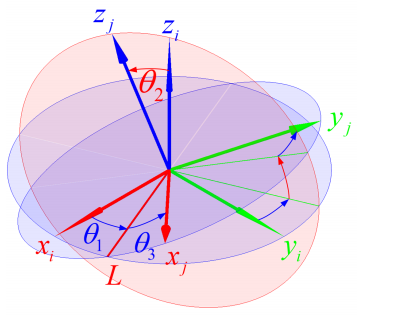
\includegraphics[width=0.80\textwidth]{Figure/体内ZXZ转动（经典欧拉角）示意图.png}
\par\vspace{0.2em}{\small\kaishu 体内ZXZ转动（经典欧拉角）示意图}
\end{center}
从 $i$ 系到 $j$ 系的相对转动解读为绕连体坐标系（动系）坐标轴的三次相继转动，转轴分别为 $Z$、$X$、$Z$，转角分别为 $\theta_1$、$\theta_2$、$\theta_3$。
\begin{enumerate}

\item $\theta_1$：转轴 $z_i$，进动角（$\psi$）

\item $\theta_2$：转轴 $L$（节线），章动角（$\theta$）

\item $\theta_3$：转轴 $z_j$，自转角（$\varphi$）

\end{enumerate}
坐标变换矩阵：
\[
\boldsymbol{A}_{ij}=\boldsymbol{A}_z(\theta_1)\boldsymbol{A}_x(\theta_2)\boldsymbol{A}_z(\theta_3).
\]
\textbf{体内ZXZ转动与坐标变换矩阵的关系} 由转角表示的坐标变换矩阵：
\begin{align*}
\boldsymbol{A}_{ij} &= \boldsymbol{A}_z(\theta_1)\boldsymbol{A}_x(\theta_2)\boldsymbol{A}_z(\theta_3)\notag\\
&= \begin{bmatrix}
\cos\theta_1 & -\sin\theta_1 & 0\\
\sin\theta_1 & \cos\theta_1 & 0\\
0 & 0 & 1
\end{bmatrix}
\begin{bmatrix}
1 & 0 & 0\\
0 & \cos\theta_2 & -\sin\theta_2\\
0 & \sin\theta_2 & \cos\theta_2
\end{bmatrix}
\begin{bmatrix}
\cos\theta_3 & -\sin\theta_3 & 0\\
\sin\theta_3 & \cos\theta_3 & 0\\
0 & 0 & 1
\end{bmatrix}\notag\\
&= \begin{bmatrix}
c_1c_3-s_1c_2s_3 & -c_1s_3-s_1c_2c_3 & s_1s_2\\
s_1c_3+c_1c_2s_3 & c_1c_2c_3-s_1s_3 & -c_1s_2\\
s_2s_3 & s_2c_3 & c_2
\end{bmatrix}.
\end{align*}
由坐标变换矩阵反求转角：
\[
\boldsymbol{A}_{ij}=
\begin{bmatrix}
c_1c_3-s_1c_2s_3 & -c_1s_3-s_1c_2c_3 & s_1s_2\\
s_1c_3+c_1c_2s_3 & c_1c_2c_3-s_1s_3 & -c_1s_2\\
s_2s_3 & s_2c_3 & c_2
\end{bmatrix}
=
\begin{bmatrix}
a_{11} & a_{12} & a_{13}\\
a_{21} & a_{22} & a_{23}\\
a_{31} & a_{32} & a_{33}
\end{bmatrix}.
\]
由上式可知：
(I) 当 $c_2=a_{33}\approx 1$ 时，$s_2\approx 0$，此时
\[
\boldsymbol{A}_{ij}=
\begin{bmatrix}
c_1c_3-s_1s_3 & -c_1s_3-s_1c_3 & 0\\
s_1c_3+c_1s_3 & c_1c_3-s_1s_3 & 0\\
0 & 0 & 1
\end{bmatrix}
=
\begin{bmatrix}
a_{11} & a_{12} & 0\\
a_{21} & a_{22} & 0\\
0 & 0 & 1
\end{bmatrix},
\]
\[
a_{11}=\cos(\theta_1+\theta_3),\qquad a_{21}=\sin(\theta_1+\theta_3).
\]
可取
\[
\theta_2=0+2k_1\pi,\qquad \theta_1+\theta_3=\mathrm{atan2}(a_{21},a_{11})+2k_2\pi.
\]
(II) 当 $c_2=a_{33}\approx -1$ 时，$s_2\approx 0$，此时
\[
\boldsymbol{A}_{ij}=
\begin{bmatrix}
c_1c_3+s_1s_3 & -c_1s_3+s_1c_3 & 0\\
s_1c_3-c_1s_3 & -c_1c_3-s_1s_3 & 0\\
0 & 0 & -1
\end{bmatrix}
=
\begin{bmatrix}
a_{11} & a_{12} & 0\\
a_{21} & a_{22} & 0\\
0 & 0 & -1
\end{bmatrix},
\]
\[
a_{11}=\cos(\theta_1-\theta_3),\qquad a_{21}=\sin(\theta_1-\theta_3).
\]
可取
\[
\theta_2=\pi+2k_1\pi,\qquad \theta_1-\theta_3=\mathrm{atan2}(a_{21},a_{11})+2k_2\pi.
\]
(III) 当 $|c_2|=|a_{33}|\neq 1$ 时，
\[
\begin{bmatrix}
1 & -a_{33}\\
a_{33} & -1
\end{bmatrix}
\begin{bmatrix}
c_1c_3\\
s_1s_3
\end{bmatrix}
=
\begin{bmatrix}
a_{11}\\
a_{22}
\end{bmatrix}
\Rightarrow
\left\{\begin{aligned}
c_1c_3 &= (a_{11}-a_{22}a_{33})/(1-a_{33}^2)=:b_1\\
s_1s_3 &= (-a_{22}+a_{11}a_{33})/(1-a_{33}^2)=:b_2
\end{aligned}\right.
\]
\[
\begin{bmatrix}
-a_{33} & -1\\
1 & a_{33}
\end{bmatrix}
\begin{bmatrix}
s_1c_3\\
c_1s_3
\end{bmatrix}
=
\begin{bmatrix}
a_{12}\\
a_{21}
\end{bmatrix}
\Rightarrow
\left\{\begin{aligned}
s_1c_3 &= (a_{21}+a_{12}a_{33})/(1-a_{33}^2)=:b_3\\
c_1s_3 &= (-a_{12}-a_{21}a_{33})/(1-a_{33}^2)=:b_4
\end{aligned}\right.
\]
\[
\left\{\begin{aligned}
\theta_1+\theta_3 &= \mathrm{atan2}(b_3+b_4,\,b_1-b_2)=:b_5+2k_1\pi\\
\theta_1-\theta_3 &= \mathrm{atan2}(b_3-b_4,\,b_1+b_2)=:b_6+2k_2\pi
\end{aligned}\right.
\quad\Rightarrow\quad
\left\{\begin{aligned}
\theta_1 &= (b_5+b_6)/2+k_3\pi\\
\theta_3 &= (b_5-b_6)/2-k_3\pi+2k_4\pi
\end{aligned}\right.
\]
\textbf{体内ZXZ转动与角速度投影列阵的关系} 由 $\tilde{\boldsymbol{\omega}}_{ij|j}=\boldsymbol{A}_{ij}^{\mathrm{T}}\dot{\boldsymbol{A}}_{ij}$ 可得：
\[
\boldsymbol{\omega}_{ij|j}=
\begin{bmatrix}
\sin(\theta_2)\sin(\theta_3) & \cos(\theta_3) & 0\\
\sin(\theta_2)\cos(\theta_3) & -\sin(\theta_3) & 0\\
\cos(\theta_2) & 0 & 1
\end{bmatrix}
\begin{bmatrix}
\dot{\theta}_1\\
\dot{\theta}_2\\
\dot{\theta}_3
\end{bmatrix}
=:\boldsymbol{H}_{\mathrm{BZXZ}}\dot{\boldsymbol{\theta}}.
\]
系数矩阵的行列式为
\[
\det(\boldsymbol{H}_{\mathrm{BZXZ}})=-\sin(\theta_2),
\]
因此，当 $\theta_2=k\pi$ 时，不存在从 $\boldsymbol{\omega}_{ij|j}$ 到 $\dot{\boldsymbol{\theta}}$ 的对应关系；也不存在从 $\dot{\boldsymbol{\omega}}_{ij|j}$ 到 $\ddot{\boldsymbol{\theta}}$ 的对应关系。$\theta_2=k\pi$ 为此类三轴角的奇异点。
角速度列阵 $\boldsymbol{\omega}_{ij|j}$ 对体内ZXZ转角 $\boldsymbol{\theta}$ 的偏导数满足
\[
\frac{\partial\boldsymbol{\omega}_{ij|j}}{\partial\boldsymbol{\theta}}=
\begin{bmatrix}
0 & \cos(\theta_2)\sin(\theta_3)\dot{\theta}_1 & \sin(\theta_2)\cos(\theta_3)\dot{\theta}_1-\cos(\theta_3)\dot{\theta}_2\\
0 & \cos(\theta_2)\cos(\theta_3)\dot{\theta}_1 & -\sin(\theta_2)\sin(\theta_3)\dot{\theta}_1-\sin(\theta_3)\dot{\theta}_2\\
0 & -\sin(\theta_2)\dot{\theta}_1 & 0
\end{bmatrix}.
\]
\subsection{体内ZYX转动（卡尔丹角，Yaw-Pitch-Roll）}
\begin{center}
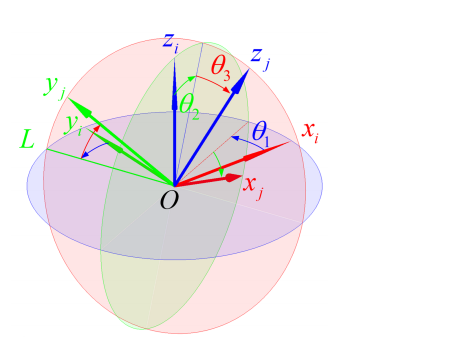
\includegraphics[width=0.80\textwidth]{Figure/SystemDynamicsModelingAndSimulation_75.png}
\par\vspace{0.2em}{\small\kaishu 体内ZYX转动（卡尔丹角）示意图}
\end{center}
从 $i$ 系到 $j$ 系的相对转动解读为绕连体坐标系（动系）坐标轴的三次相继转动，转轴分别为 $Z$、$Y$、$X$，转角分别为 $\theta_1$、$\theta_2$、$\theta_3$。
\begin{enumerate}

\item $\theta_1$：转轴 $z_i$，偏航角（$\psi$）

\item $\theta_2$：转轴 $L$（节线），俯仰角（$\theta$）

\item $\theta_3$：转轴 $x_j$，滚转角（$\varphi$）

\end{enumerate}
坐标变换矩阵：
\[
\boldsymbol{A}_{ij}=\boldsymbol{A}_z(\theta_1)\boldsymbol{A}_y(\theta_2)\boldsymbol{A}_x(\theta_3).
\]
\textbf{体内ZYX转动与坐标变换矩阵的关系} 由转角表示的坐标变换矩阵：
\begin{align*}
\boldsymbol{A}_{ij} &= \boldsymbol{A}_z(\theta_1)\boldsymbol{A}_y(\theta_2)\boldsymbol{A}_x(\theta_3)\notag\\
&= \begin{bmatrix}
\cos\theta_1 & -\sin\theta_1 & 0\\
\sin\theta_1 & \cos\theta_1 & 0\\
0 & 0 & 1
\end{bmatrix}
\begin{bmatrix}
\cos\theta_2 & 0 & \sin\theta_2\\
0 & 1 & 0\\
-\sin\theta_2 & 0 & \cos\theta_2
\end{bmatrix}
\begin{bmatrix}
1 & 0 & 0\\
0 & \cos\theta_3 & -\sin\theta_3\\
0 & \sin\theta_3 & \cos\theta_3
\end{bmatrix}\notag\\
&= \begin{bmatrix}
c_1c_2 & -s_1c_3+c_1s_2s_3 & s_1s_3+c_1s_2c_3\\
s_1c_2 & c_1c_3+s_1s_2s_3 & -c_1s_3+s_1s_2c_3\\
-s_2 & c_2s_3 & c_2c_3
\end{bmatrix}.
\end{align*}
由坐标变换矩阵反求转角：
\[
\boldsymbol{A}_{ij}=
\begin{bmatrix}
c_1c_2 & -s_1c_3+c_1s_2s_3 & s_1s_3+c_1s_2c_3\\
s_1c_2 & c_1c_3+s_1s_2s_3 & -c_1s_3+s_1s_2c_3\\
-s_2 & c_2s_3 & c_2c_3
\end{bmatrix}
=
\begin{bmatrix}
a_{11} & a_{12} & a_{13}\\
a_{21} & a_{22} & a_{23}\\
a_{31} & a_{32} & a_{33}
\end{bmatrix}.
\]
由上式可知：
(I) 当 $s_2=-a_{31}\approx 1$ 时，$c_2\approx 0$，此时
\[
\boldsymbol{A}_{ij}=
\begin{bmatrix}
0 & -s_1c_3+c_1s_3 & s_1s_3+c_1c_3\\
0 & c_1c_3+s_1s_3 & -c_1s_3+s_1c_3\\
-1 & 0 & 0
\end{bmatrix}
=
\begin{bmatrix}
0 & a_{12} & a_{13}\\
0 & a_{22} & a_{23}\\
-1 & 0 & 0
\end{bmatrix},
\]
\[
a_{23}=\sin(\theta_1-\theta_3),\qquad a_{22}=\cos(\theta_1-\theta_3).
\]
可取
\[
\theta_2=\pi/2+2k_1\pi,\qquad \theta_1-\theta_3=\mathrm{atan2}(a_{23},a_{22})+2k_2\pi.
\]
(II) 当 $s_2=-a_{31}\approx -1$ 时，$c_2\approx 0$，此时
\[
\boldsymbol{A}_{ij}=
\begin{bmatrix}
0 & -s_1c_3-c_1s_3 & s_1s_3-c_1c_3\\
0 & c_1c_3-s_1s_3 & -c_1s_3-s_1c_3\\
1 & 0 & 0
\end{bmatrix}
=
\begin{bmatrix}
0 & a_{12} & a_{13}\\
0 & a_{22} & a_{23}\\
1 & 0 & 0
\end{bmatrix},
\]
\[
a_{23}=-\sin(\theta_1+\theta_3),\qquad a_{22}=\cos(\theta_1+\theta_3).
\]
可取
\[
\theta_2=-\pi/2+2k_1\pi,\qquad \theta_1+\theta_3=\mathrm{atan2}(-a_{23},a_{22})+2k_2\pi.
\]
(III) 当 $|s_2|=|a_{31}|\neq 1$ 时，
\[
\begin{bmatrix}
1 & -a_{31}\\
-a_{31} & 1
\end{bmatrix}
\begin{bmatrix}
c_1c_3\\
s_1s_3
\end{bmatrix}
=
\begin{bmatrix}
a_{22}\\
a_{13}
\end{bmatrix}
\Rightarrow
\left\{\begin{aligned}
c_1c_3 &= (a_{22}+a_{13}a_{31})/(1-a_{31}^2)=:b_1\\
s_1s_3 &= (a_{13}+a_{22}a_{31})/(1-a_{31}^2)=:b_2
\end{aligned}\right.
\]
\[
\begin{bmatrix}
-a_{31} & -1\\
-1 & -a_{31}
\end{bmatrix}
\begin{bmatrix}
s_1c_3\\
c_1s_3
\end{bmatrix}
=
\begin{bmatrix}
a_{23}\\
a_{12}
\end{bmatrix}
\Rightarrow
\left\{\begin{aligned}
s_1c_3 &= (-a_{12}+a_{23}a_{31})/(1-a_{31}^2)=:b_3\\
c_1s_3 &= (-a_{23}+a_{12}a_{31})/(1-a_{31}^2)=:b_4
\end{aligned}\right.
\]
\[
\left\{\begin{aligned}
\theta_1+\theta_3 &= \mathrm{atan2}(b_3+b_4,\,b_1-b_2)=:b_5+2k_1\pi\\
\theta_1-\theta_3 &= \mathrm{atan2}(b_3-b_4,\,b_1+b_2)=:b_6+2k_2\pi
\end{aligned}\right.
\quad\Rightarrow\quad
\left\{\begin{aligned}
\theta_1 &= (b_5+b_6)/2+k_3\pi\\
\theta_3 &= (b_5-b_6)/2-k_3\pi+2k_4\pi
\end{aligned}\right.
\]
\textbf{体内ZYX转动与角速度投影列阵的关系} 由 $\tilde{\boldsymbol{\omega}}_{ij|j}=\boldsymbol{A}_{ij}^{\mathrm{T}}\dot{\boldsymbol{A}}_{ij}$ 可得：
\[
\boldsymbol{\omega}_{ij|j}=
\begin{bmatrix}
-\sin(\theta_2) & 0 & 1\\
\cos(\theta_2)\sin(\theta_3) & \cos(\theta_3) & 0\\
\cos(\theta_2)\cos(\theta_3) & -\sin(\theta_3) & 0
\end{bmatrix}
\begin{bmatrix}
\dot{\theta}_1\\
\dot{\theta}_2\\
\dot{\theta}_3
\end{bmatrix}
=:\boldsymbol{H}_{\mathrm{BZYX}}\dot{\boldsymbol{\theta}}.
\]
系数矩阵的行列式为
\[
\det(\boldsymbol{H}_{\mathrm{BZYX}})=-\cos(\theta_2),
\]
因此，当 $\theta_2=\pi/2+k\pi$ 时，不存在从 $\boldsymbol{\omega}_{ij|j}$ 到 $\dot{\boldsymbol{\theta}}$ 的对应关系；也不存在从 $\dot{\boldsymbol{\omega}}_{ij|j}$ 到 $\ddot{\boldsymbol{\theta}}$ 的对应关系。$\theta_2=\pi/2+k\pi$ 为此类三轴角的奇异点。
角速度列阵 $\boldsymbol{\omega}_{ij|j}$ 对体内ZYX转角 $\boldsymbol{\theta}$ 的偏导数满足
\[
\frac{\partial\boldsymbol{\omega}_{ij|j}}{\partial\boldsymbol{\theta}}=
\begin{bmatrix}
0 & -\cos(\theta_2)\dot{\theta}_1 & 0\\
0 & -\sin(\theta_2)\sin(\theta_3)\dot{\theta}_1 & \cos(\theta_2)\cos(\theta_3)\dot{\theta}_1-\sin(\theta_3)\dot{\theta}_2\\
0 & -\sin(\theta_2)\cos(\theta_3)\dot{\theta}_1 & -\cos(\theta_2)\sin(\theta_3)\dot{\theta}_1-\cos(\theta_3)\dot{\theta}_2
\end{bmatrix}.
\]
\section{坐标系姿态广义坐标的其他形式}
\begin{enumerate}

\item \textbf{旋转向量/罗德里格斯向量}

\end{enumerate}
\[
\boldsymbol{\rho}=\theta\boldsymbol{n}.
\]
\begin{enumerate}

\item \textbf{罗德里格斯参数/吉布斯向量}（Rodrigues parameters / Gibbs vector）

\end{enumerate}
\[
\boldsymbol{g}=\boldsymbol{n}\tan\frac{\theta}{2}.
\]
\begin{enumerate}

\item \textbf{修正的罗德里格斯参数}（Modified Rodrigues Parameters, MRP）

\end{enumerate}
\[
\boldsymbol{\sigma}=\boldsymbol{n}\tan\frac{\theta}{4}.
\]
\section{相继转动}
\textbf{方向余弦矩阵与转轴转角的关系} 用转轴和转角表示的方向余弦矩阵：
\[
\boldsymbol{A}_{ij}=\boldsymbol{I}_3\cos\theta+\tilde{\boldsymbol{n}}\sin\theta+\boldsymbol{n}\boldsymbol{n}^{\mathrm{T}}(1-\cos\theta).
\]
当转轴 $\boldsymbol{n}$ 相对于 $i$ 系和 $j$ 系固定时，
\[
\dot{\boldsymbol{A}}_{ij}=(-\boldsymbol{I}_3\sin\theta+\tilde{\boldsymbol{n}}\cos\theta+\boldsymbol{n}\boldsymbol{n}^{\mathrm{T}}\sin\theta)\,\dot{\theta}.
\]
接下来对
\begin{align*}
\tilde{\boldsymbol{\omega}}_{ij|j} &= \boldsymbol{A}_{ij}^{\mathrm{T}}\dot{\boldsymbol{A}}_{ij}\notag\\
&= \left[\boldsymbol{I}_3\cos\theta+\tilde{\boldsymbol{n}}^{\mathrm{T}}\sin\theta+\boldsymbol{n}\boldsymbol{n}^{\mathrm{T}}(1-\cos\theta)\right](-\boldsymbol{I}_3\sin\theta+\tilde{\boldsymbol{n}}\cos\theta+\boldsymbol{n}\boldsymbol{n}^{\mathrm{T}}\sin\theta)\,\dot{\theta}
\end{align*}
进行化简。
\begin{proof}[化简过程]
利用角速度矢量列阵的叉乘矩阵关系 $\tilde{\boldsymbol{n}}\tilde{\boldsymbol{n}}=\boldsymbol{n}\boldsymbol{n}^{\mathrm{T}}-\boldsymbol{I}_3$：

\begin{align*}
\tilde{\boldsymbol{\omega}}_{ij|j} &= \boldsymbol{A}_{ij}^{\mathrm{T}}\dot{\boldsymbol{A}}_{ij}\notag\\
&= \left[\boldsymbol{I}_3\cos\theta+\tilde{\boldsymbol{n}}^{\mathrm{T}}\sin\theta+\boldsymbol{n}\boldsymbol{n}^{\mathrm{T}}(1-\cos\theta)\right](-\boldsymbol{I}_3\sin\theta+\tilde{\boldsymbol{n}}\cos\theta+\boldsymbol{n}\boldsymbol{n}^{\mathrm{T}}\sin\theta)\,\dot{\theta}\notag\\
&= (-\boldsymbol{I}_3\sin\theta\cos\theta+\tilde{\boldsymbol{n}}\cos^2\theta+\boldsymbol{n}\boldsymbol{n}^{\mathrm{T}}\sin\theta\cos\theta)\,\dot{\theta}\notag\\
&\quad + \left(-\tilde{\boldsymbol{n}}^{\mathrm{T}}\sin^2\theta+\tilde{\boldsymbol{n}}^{\mathrm{T}}\tilde{\boldsymbol{n}}\sin\theta\cos\theta+\tilde{\boldsymbol{n}}^{\mathrm{T}}\boldsymbol{n}\boldsymbol{n}^{\mathrm{T}}\sin^2\theta\right)\dot{\theta}\notag\\
&\quad + \left[-\boldsymbol{n}\boldsymbol{n}^{\mathrm{T}}\sin\theta(1-\cos\theta)+\boldsymbol{n}\boldsymbol{n}^{\mathrm{T}}\tilde{\boldsymbol{n}}\cos\theta(1-\cos\theta)+\boldsymbol{n}\boldsymbol{n}^{\mathrm{T}}\boldsymbol{n}\boldsymbol{n}^{\mathrm{T}}\sin\theta(1-\cos\theta)\right]\dot{\theta}\notag\\
&= \tilde{\boldsymbol{n}}(\cos^2\theta+\sin^2\theta)\dot{\theta}\notag\\
&\quad + \left[-\boldsymbol{I}_3+\boldsymbol{n}\boldsymbol{n}^{\mathrm{T}}-(\boldsymbol{n}\boldsymbol{n}^{\mathrm{T}}-\boldsymbol{I}_3)\right]\sin\theta\cos\theta\,\dot{\theta}\notag\\
&= \tilde{\boldsymbol{n}}\dot{\theta}\notag\\
&= \widetilde{\boldsymbol{n}\dot{\theta}}.
\end{align*}
\end{proof}
由此可知
\begin{theorem}[固定转轴的角速度]
当转轴 $\boldsymbol{n}$ 相对于 $i$ 系和 $j$ 系固定时，

\[
\boldsymbol{\omega}_{ij|j}=\boldsymbol{n}\dot{\theta}.
\]
\end{theorem}
此时
\begin{align*}
\boldsymbol{\omega}_{ij|i} &= \boldsymbol{A}_{ij}\boldsymbol{\omega}_{ij|j}\notag\\
&= \left[\boldsymbol{I}_3\cos\theta+\tilde{\boldsymbol{n}}\sin\theta+\boldsymbol{n}\boldsymbol{n}^{\mathrm{T}}(1-\cos\theta)\right]\boldsymbol{n}\dot{\theta}\notag\\
&= \boldsymbol{n}\dot{\theta}=\boldsymbol{\omega}_{ij|j}.
\end{align*}
当涉及多次相对转动时，为避免歧义，以上两式又可记为
\[
\boldsymbol{\omega}_{ij|i}=\boldsymbol{\omega}_{ij|j}=\boldsymbol{n}_{ij}\dot{\theta}_{ij}.
\]
设 $l$ 系由 $i$ 系经三次相继转动获得，相应的方向余弦矩阵表示为
\[
\boldsymbol{A}_{il}=\boldsymbol{A}_{ij}(\boldsymbol{n}_{ij},\theta_{ij})\boldsymbol{A}_{jk}(\boldsymbol{n}_{jk},\theta_{jk})\boldsymbol{A}_{kl}(\boldsymbol{n}_{kl},\theta_{kl}),
\]
且 $\boldsymbol{n}_{ij}$、$\boldsymbol{n}_{jk}$、$\boldsymbol{n}_{kl}$ 不随时间变化。此时，上式对时间的一阶导数可表示为
\[
\boldsymbol{A}_{il}\tilde{\boldsymbol{\omega}}_{il|l}
=\boldsymbol{A}_{ij}\tilde{\boldsymbol{\omega}}_{ij|j}\boldsymbol{A}_{jk}\boldsymbol{A}_{kl}
+\boldsymbol{A}_{ij}\boldsymbol{A}_{jk}\tilde{\boldsymbol{\omega}}_{jk|k}\boldsymbol{A}_{kl}
+\boldsymbol{A}_{ij}\boldsymbol{A}_{jk}\boldsymbol{A}_{kl}\tilde{\boldsymbol{\omega}}_{kl|l},
\]
式中
\[
\boldsymbol{\omega}_{ij|j}=\boldsymbol{n}_{ij}\dot{\theta}_{ij},\qquad
\boldsymbol{\omega}_{jk|k}=\boldsymbol{n}_{jk}\dot{\theta}_{jk},\qquad
\boldsymbol{\omega}_{kl|l}=\boldsymbol{n}_{kl}\dot{\theta}_{kl}.
\]
则
\begin{theorem}[相继转动的角速度合成]
\[
\boldsymbol{\omega}_{il|l}
=\boldsymbol{A}_{lj}\boldsymbol{\omega}_{ij|j}+\boldsymbol{A}_{lk}\boldsymbol{\omega}_{jk|k}+\boldsymbol{\omega}_{kl|l}
=\boldsymbol{A}_{lj}\boldsymbol{n}_{ij}\dot{\theta}_{ij}+\boldsymbol{A}_{lk}\boldsymbol{n}_{jk}\dot{\theta}_{jk}+\boldsymbol{n}_{kl}\dot{\theta}_{kl}.
\]

（教材原书写作 $\boldsymbol{\omega}_{il|l}=\boldsymbol{A}_{jl}^{\mathrm{T}}\boldsymbol{\omega}_{ij|j}+\boldsymbol{A}_{kl}^{\mathrm{T}}\boldsymbol{\omega}_{jk|k}+\boldsymbol{\omega}_{kl|l}$，其中 $\boldsymbol{A}_{jl}^{\mathrm{T}}=\boldsymbol{A}_{lj}$、$\boldsymbol{A}_{kl}^{\mathrm{T}}=\boldsymbol{A}_{lk}$，即把各段角速度的投影列阵变换到 $l$ 系后叠加。）
\end{theorem}
